\documentclass[../thesis.tex]{subfiles}
\begin{document}

\chapter{Errors and Limits}
\label{chp:err_lims}

Within this section the errors and limitations of the build model are looked at.

\section{Errors}

The models solution is an iterative procedure as described in \autoref{sec:sol_method}. Within this process the solution obtained within one iteration is used as initial starting point for the next one. The procedure also involves a correction step as shown for the pressure and velocity field in \autoref{fig:PISO}. These corrections can be tracked over the iterations done throughout the simulation run. The results also called \texttt{residuals} can be seen in \autoref{fig: residuals}.
\begin{figure}[htbp]
	\centering
	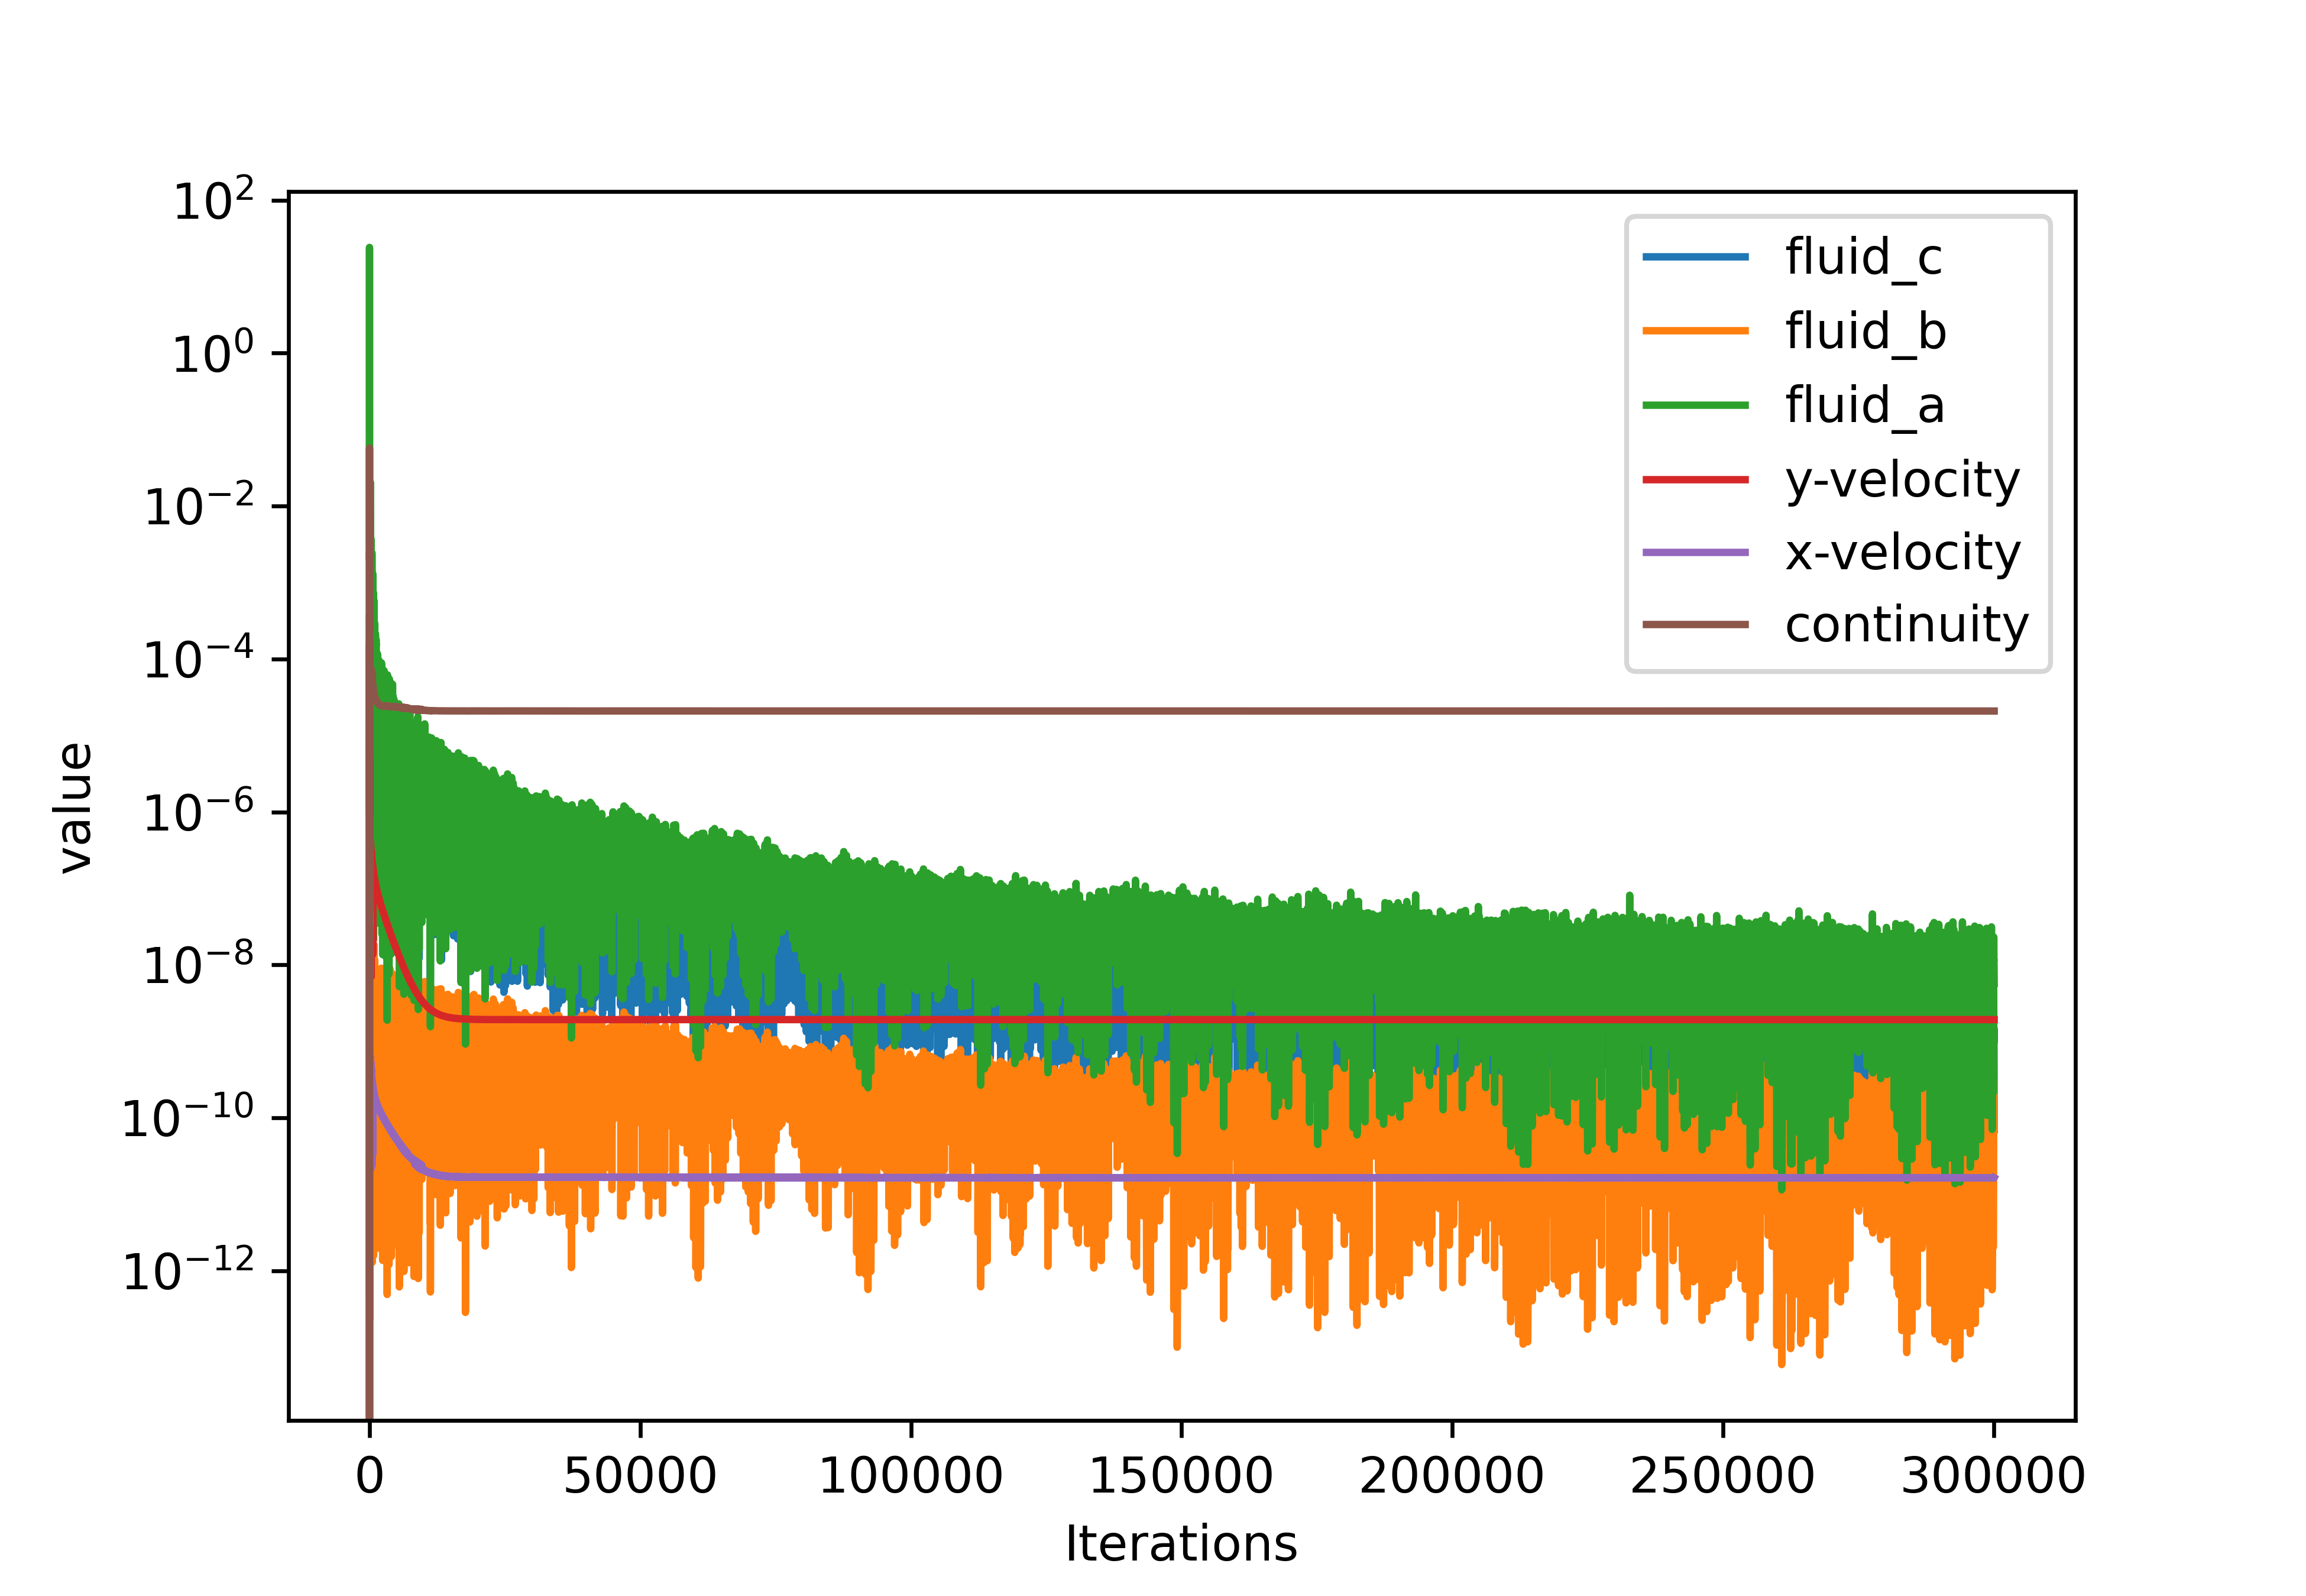
\includegraphics[width=\textwidth]{residuals_h2r3_P500E2_S120E4}
	\caption{example residuals plot}
	\label{fig: residuals}
\end{figure}
To check that the model has converged for a solution step thresholds for the residuals are set. If the residual value for a variable is below the set threshold the solution has converged and the next step is performed. From the plot it can be seen that the residuals do have values of $10^{-5}$ and below so the model performs well for the given example. The values do jump up and down a bit for certain variables that is due to the moving flow and changing fluid composition resulting from the reaction. For the continuity and velocity variables the residuals are represented by a straight line because once the velocity field is established it does not change any more.

The residuals give an indication on the model's errors and can be used as well to check if the model behaves correctly or which part has to be changed if the solution does not converge or other errors occur.

\section{Limitations}
\label{sec: lim_improv}
Throughout the model's development process some limitations can be determined that are described in this section.

In its current state the model can not be run for Peclet-Numbers way higher than the highest investigated which has a value of $2050$. If the Peclet-Number is increased the input velocity goes up as well if the Schmidt-Number is not touched. A higher input velocity needs a lower time step and sometimes a finer mesh to resolve all necessary fluid phenomena happening. Both changes drive up the simulation time exponentially so the amount of computational resources needed for obtaining results in a reasonable amount of time goes way up. Since computational resources are not unlimited it's a good practice to create a combination of mesh and solver settings that are coarse enough to show the things that need to be investigated. In addition to that the results should show a physically correct behaviour. This is not the case when increasing the Peclet-Number with the used mesh and settings. The method shown in \autoref{sec: mesh_dep} is one way to get the final mesh but the approach could still be improved. Some finer element size reduction could be implemented to get as close to the best suited mesh as possible. 

Another limitation is that the model is only using not miscible fluid components. In a real experiment all species taking part within the reaction are miscible in each other to a certain extend. To take that into account the model's species could be updated and improved or a mixture model could be needed dependent on how mixing is implemented in \texttt{ANSYS FLUENT}.

\chapter{Outlook and Conclusion}
\label{chp:out_con}
In this work a numerical model simulating a reaction diffusion advection front within a radial reactor was created. The implementation was done using the software \texttt{ANSYS FLUENT}. The model validation was performed successfully using existing experimental data. A parametric study was done starting to investigate the influence of the reactor's geometry and other input variables on the front's behaviour. Besides the front positions and the front's width, the total product formed was investigated. The changes of these variables dependent on the input settings were discussed in greater detail and the errors and limitations of the model in it's current state were mentioned.

All in all the model development and implementation was successful. The implementation and post processing is setup in a way that can easily be modified for the existing geometry or be applied to other models created in \texttt{ANSYS FLUENT} that are similar to the one used in this work. The model delivers more insight into the phenomenon of reaction-diffusion-advection fronts and provides information otherwise not accessible to experimental setups by giving a cross section view of the reactor. The possibility of running cases in parallel could help reduce the amount of experiments needed in the future. The model could also be used for validating existing experimental runs. Since experiments under 0g conditions are monetary expensive and consume a lot of time for preparation and data processing the developed model provides a resource efficient alternative. Further research could be done on the influence of different input concentrations on the fronts metrics or the influence of the reaction speed could be looked at to give a few possibilities for further investigations. 

The developed model sets a step in the direction to gain further understanding on what is happening at the front's formation process at early time stages under 0g conditions. A foundation is laid in this work that can be used for further research and investigations.

\end{document}